% Document settings:

\documentclass[12pt]{article}
\linespread{1.6}
\usepackage[margin=1.0in]{geometry}
\usepackage{graphicx}
\usepackage{wrapfig}
\usepackage{setspace}
\usepackage{wasysym}
% \graphicspath{ {/Users/bsevans/Desktop/gits/isotopes/} }

% Header information:

\singlespace \title{\Large \linespread{0} The ``urban-\emph{adapted}'' bird: Does dietary plasticity allow some species of birds to thrive in urban habitats?}
% \author{\normalsize Brian S. Evans} 
\date{}

% Start: 
\begin{document}
\maketitle \vspace{-2cm}

% Background: 

\doublespace
\noindent {\textbf {1. BACKGROUND}}: Urbanization has altered habitats, restructured avian communities, and influenced the range sizes and population dynamics of hundreds of bird species [1-3]. While urban environments comprise just 5.6 percent of the total land cover of the United States[4], the shift from rural to urban land use is considered to be the second leading cause of species endangerment and extinction during the twentieth century[5]. As the proportion of developed land is projected to increase by as much as 63 percent in the first half of this century[6], urbanization is expected to become the primary driver of species extinction and thus understanding how organisms respond to urban habitats is of paramount importance[2]. Despite the urgency to minimize the impacts of urbanization, our ability to apply effective conservation strategies is hindered by a limited understanding of the mechanisms by which urban habitats influences bird populations [7]. \par

The interaction between human land use and the life history traits of species determines whether a given species will be a ``winner" (urban-adapted species) or ``loser" in human-dominated landscapes (urban-avoiding species)[1,8]. It is hypothesized that bird populations and communities in anthropogenic environments are largely structured by the distribution of resources accessible to a given dietary guild[9,10]. Species with specialist dietary requirements, especially obligate insectivores[11], are expected to be sensitive to human-induced habitat modification and may therefore experience high rates of local extinction across the urban habitat matrix[12]. Conversely, species with generalist dietary habitats and those that have the ability to use anthropogenic resources (e.g., granivores using bird feeders[13]) are expected to be positively associated with urban environments[1]. For example, urban landscapes dominated by ornamental and non-native species provide essential resources for frugivorous birds, especially during winter months[14], but are expected to negatively influence insectivores due to reduced abundances of insects during the growing season[15]. While studies of avian community composition[16] and survival[10] suggest the influence of resources on avian response, the direct connection between avian health and the use of resources across the rural-to-urban gradient has not yet been empirically tested.\par

In proposed research, I seek to examine the influence of urban land cover on avian diet and condition across the rural-to-urban gradient at local and regional scales in metropolitan Washington D.C. I expect that the composition and abundance of avian food resources vary temporally and spatially along this gradient with resource subsidization as the primary driver of higher food availability at intermediate degrees of urbanization[17,18]. As such, I expect that the maintainance of populations in urban environments is contingent on the ability to utilize these resources. Specifically, the proposed research will address:  1) Do birds vary their diet across the rural-to-urban gradient? 2) Do birds exhibit increased omnivory with increasing urban land cover? 3) What are the consequences of diet on bird health in  urban environments? 4) Do local-scale habitat features moderate the influence of urbanization on avian diet and health? \par

To address these questions, I will take feather and claw samples from birds across the rural-to-urban gradient and measure the stable isotope ratios of Carbon and Nitrogen to assess avian diet and concentrations of the stress hormone corticosterone (CORT) as an index of the condition of individuals. CORT has been found to be predictive of several biologically important indicators of bird health, with low CORT values associated with breeding success[19], body condition[20], and survival[21]. Analysis of stable isotope ratios of $\delta^{13}$C and $\delta^{15}$N has been applied to estimate the trophic position of prey items in feather[22,23] and claw [24] material. Tail feathers are molted immediately following the end of the breeding cycle and thus $\delta^{13}$C and $\delta^{15}$N ratios represent a snapshot of an individual's diet during the growth of the feather. While claw material is grown continuously, samples collected at the start of the breeding season are representative of bird diet prior to the breeding period. As feather and claw samples are representative of avian diet at different points in a bird's annual cycle, assessing isotopic ratios within both claw and feather samples provides a key temporal signature of avian diet [25] and allows researchers to assess the width of a bird's dietary niche [24,26]. The combined analysis of $\delta^{13}$C, $\delta^{15}$N, and CORT in feather and claw samples allows us to evaluate relationship between urbanization, dietary niche, and the relationship between diet and avian health [27].\par

% PROPOSED RESEARCH

\noindent {\textbf {3. PROPOSED RESEARCH}}: I propose to assess variation in diet and condition across the rural-to-urban gradient in two species of birds: the Northern Cardinal (NOCA, \textit{Cardinalis cardinalis}) and Carolina Chickadee (CACH, \textit{Poecile carolinensis}). Differences and similarities in the life histories of these species, both of which are common to the rural and suburban habitats of metropolitan Washington, D.C., provide an ideal study system with which to assess the influence of urbanization on avian diet and health. Both species exhibit some degree of omnivory, are non-migratory, and utilize bird feeders in suburban and urban habitats. Key differences between the life history of the species include nesting habits (NOCA are cup nesting and CACH cavity nesting species) and response to urbanization (NOCA are found at more urban sites than CACH). % GENERAL METHODS

\noindent \underline{GENERAL METHODS}. \textit {Field sampling}: This study will utilize data collected as a part of the Neighborhood Nestwatch Program (NN), a citizen science project run by the Smithsonian Migratory Bird Center. NN has established a network of over 200 sampling sites within metropolitan Washington D.C., with sampling predominantly located at the homes of project participants. Habitats represented by study sites range from rural open and forested areas, to suburban and urban environments. Technicians will visit participant properties at the start of avian breeding season and capture birds using target netting. Tail feather and claw samples will be taken from adult male birds (n = 50 of each species). All potential dietary sources, including samples available fruits, arthropods, and supplemental food sources, will be collected from sites and their surrounding areas ($\leq$ 100 m) at three periods over the course of a year -- during the banding visit, at the end of the breeding season, and during winter months. \textit{Stable Isotopes and CORT}: Samples of potential dietary sources will be dried in ovens prior to analysis. All samples will be washed in a 2:1 chloroform:methanol solution to remove surface oils and combusted at 1350$^{\circ}$C in an elemental analyzer and analyzed in a continuous-flow isotope ratio mass spectrometer following the methods of Rushing et al.[29]. Isotopic ratios $^{13}$C and $^{15}$C will be evaluated relative to the Pee Dee Belemnite and atmospheric nitrogen standards, respectively, and reported per mil using $\delta$ notation using the equation: $\delta{X} = (R_{sample}/R_{standard} -1) \times 1000\permil$. Accuracy and precision of $\delta^{13}$C and $\delta^{15}$N is expected to be within $\pm 2.0 \permil$[30]. We will use the Bayesian stable isotope mixing model (SIMM) of Hopkins and Ferguson[31] to evaluate the proportional composition of dietary sources for each individual. To examine the adult condition of birds, we will measure CORT in feather and claw samples using a methanol based extraction, modified from Bortolotti et al.[32], and a commercial ELISA kit (Corticosterone ELISA kit; Neogen Corporation, Ayr, UK) following Carbajal et al.[33]. \textit{Local and regional habitat variables}: I will assess the variation in $\delta^{13}$C,  $\delta^{15}$N, and CORT as a function of local and regional scale habitat features. Regional habitat features include the proportion of impervious surface and canopy cover within 500 and 1000 m of a given site to approximate the position of the site along the rural-to-urban gradient. These proxy variable and scales of analysis have been shown to be predictive of a demographic response in birds to urban land cover[10,34]. Local habitat features, sampled at NN sites between 2010 and 2015, include shrub cover, canopy height and proportional cover, and ground cover. Additional local-scale habitat features will be derived from participant surveys and include supplemental feeding habits (i.e., presence and maintenance of bird feeders) and the presence or absence of outdoor cats and dogs. It is expected that some local habitat features (e.g., shrub cover) buffer the response of birds to urbanization while others (e.g., free-roaming cats) negatively influence avian health in urban habitats [35]. \textit{Analysis}: I will use Structural Equation Modeling (SEM[36]) to examine hypothesized relationships between habitat features, bird health, and dietary habits (stable isotopes, below). SEM is a multivariate technique that allows us to simultaneously analyze the complex, and often correlated, inter-relationships among measured (e.g., CORT and land-cover) and latent variables (i.e., those estimated from measured values such as niche width). I will use a Bayesian framework to develop and test \textit{a priori} SEM in JAGS, implemented in Program R[37]. I will evaluate the influence of structural linkages between local and regional scale environmental attributes, CORT, and dietatry traits using Markov chain Monte Carlo sampling and use Bayesian model selection to compare \textit{a priori} models[38]. 
\begin{wrapfigure}{l}{0.3\textwidth}
   \centering
    \includegraphics[width=0.3\textwidth]{predictionsPlot}
\end{wrapfigure}
% HYPOTHESES AND PREDICTIONS
\noindent \underline{PREDICTIONS}. We hypothesize that \noindent{\textbf{the condition of birds is influenced by variation in the composition and breadth of the dietary habits of conspecific birds across the rural-to-urban gradient.}} \underline{Prediction 1}: \textit{The ratios of $\delta^{13}$C and $\delta^{15}$N in feathers will reflect dietary shifts from insect to plant-based and anthropogenic food sources.}  SIMMs of $\delta^{13}$C and  $\delta^{15}$N in feather, claw, and potential food items provide an estimate of the proportional composition of plant-based foods and insects in the diet. We expect that, with increasing urbanization the ratio of insects to plant-based foods, especially anthropogenic food sources, will decline. Furthermore, we expect that NOCA will exhibit higher dietary plasticity than CACH due to differential rates of in decline abundance between these species across the rural-to-urban gradient in Washington D.C.[28]. \underline{Prediction 2}: \textit{The dietary niche width among conspecifics will increase with increasing urban land cover.} Combined claw and tissue samples provide a measure of individual variance in dietary habits. Species with higher degrees of dietary specialization are expected to exhibit low variance in $\delta$-values[39]. We will use dietary estimates obtained from SIMMs to evaluate dietary diversity using the Shannon-Weiner as a metric of niche width[26]. As above, we expect that NOCA exhibits a wider niche breadth relative to CACH. \underline{Prediction 3}: \textit{Avian condition decreases with increasing omnivory for NOCA but not CACH.} Survival of NOCA was shown to increase across the rural-to-urban gradient in Washington, D.C. while urban land cover had no measurable effect on CACH survival [10]. Using CORT as a proxy of avian condition, we expect that urban environments are beneficial for species exhibiting high dietary plasticity (NOCA) but not those exhibiting low plasticity (e.g., CACH). Additionally, we expect that CORT concentrations will be especially responsive to local rather than regional habitat variables. For example, preliminary analysis of CORT in CACH feathers at NN sites (n = 22) revealed elevated CORT concentrations in sites dominated by non-native plants ($\beta$ = -3.2 $\pm$ 1.4, p-value = 0.04) but no response to the degree of urbanization at a given site (proportion of impervious surface within 500 m, $\beta$ = 0.2 $\pm$ 0.3, p-value = 0.47). 

% PROJECT RELEVANCE

\noindent {\textbf {4. RELEVANCE OF THE PROPOSED RESEARCH}}: 
My previous research has addressed the influence of urbanization on avian dispersal [28], community composition [28], and survival [34,10] in metropolitan Washington, D.C. Despite emergent patterns that have clearly demonstrated by these studies, the influence of urban habitat on these biological processes, the mechanisms driving these patterns remain largelly unknown. By addressing the distribution and influence of resources in avian diet, the proposed research project builds upon my previous work by addressing the mechanism by which urbanization is expected to have the greatest impact on bird populations. This study will greatly expand our understanding of how urban environments shape wildlife populations and communities.

% ROLE OF SMITHSONIAN

\noindent {\textbf {5. ROLE OF THE SMITHSONIAN INSTITUTION}}:
The Smithsonian Migratory Bird Center's NN project provides unprecedented access to suburban and urban matrix  and therefore is unmatched in its ability to assess the impacts of urbanization on wildlife. Dr. Peter Marra, who developed NN, will serve as my principle advisor for this work. The ability to interact on a regular basis with Dr. Marra, an expert in using stable isotope analysis, urban ecology and migratory birds, will be invaluable to completing this study and preparing manuscripts. In addition, I will benefit from interacting regularly with Dr. Brandt Ryder and Dr. Scott Sillett.  Furthermore, the facilities available, specifically the mass-spectrometry lab in Suitland, are integral to completing the research outlined in this proposal.
\end{document}

